% PanAfriCon AI 2026 camera-ready manuscript
% Springer LNCS / CCIS (llncs.cls)
\documentclass[runningheads]{llncs}

% Force A4 PDF page size (Windows/MiKTeX otherwise defaults to Letter).
\setlength{\paperheight}{297mm}
\setlength{\paperwidth}{210mm}
\pdfpageheight=\paperheight
\pdfpagewidth=\paperwidth

\usepackage[T1]{fontenc}
\usepackage{lmodern}
\usepackage{graphicx}
\usepackage{amsmath,amssymb}
\usepackage{booktabs}
\usepackage{xcolor}
\usepackage{url}
\usepackage{placeins}
\usepackage{enumitem}
\setlist[itemize]{leftmargin=*,itemsep=0.2em,topsep=0.35em,label=\textbullet}

\usepackage{flafter}
\renewcommand{\textfraction}{0.08}
\renewcommand{\topfraction}{0.92}
\renewcommand{\bottomfraction}{0.85}
\renewcommand{\floatpagefraction}{0.90}
\setcounter{totalnumber}{4}
\setcounter{topnumber}{2}
\setcounter{bottomnumber}{2}

\begin{document}
\raggedbottom

\title{Beyond Detection Parity: Localization Parity in Pedestrian Detection}
\titlerunning{Beyond Detection Parity: Localization Parity}
\authorrunning{Adissu et al.}

\author{Abel Adissu \and
Anwar Gashaw Yimam \and
Dawit Kindea \and
Beakal Gizachew \and
Elefelious Getachew}
\institute{Addis Ababa University, Addis Ababa, Ethiopia\\
\email{abel.adissu-ug@aau.edu.et,
anwar.gashaw-ug@aau.edu.et,
dawit.kindea-ug@aau.edu.et,
beakal.gizachew@aau.edu.et,
elefelious.getachew@aau.edu.et}}

\maketitle

\begin{abstract}
Pedestrian detection is a safety-critical component of autonomous driving and
intelligent surveillance, where equitable performance across demographic groups
is essential for trustworthy deployment. Fairness research in this domain has
evaluated performance almost exclusively through detection recall, that is,
whether a person is found at all, leaving the precision of the predicted
bounding box unexamined. Because existing audits reduce localization to a binary
hit-or-miss threshold, systematic disparities in how tightly detectors localize
different groups remain invisible, even though loose boxes directly compromise
downstream distance and trajectory estimates. This paper introduces
\emph{Localization Parity}, a fairness criterion that requires equal expected
Intersection over Union across demographic groups conditional on detection. We
present the first confounder-controlled audit spanning four driving datasets
(BDD100K, CityPersons, EuroCity-Day, and EuroCity-Night), three detector
families (YOLOX, RetinaNet, and Cascade~R-CNN), and two demographic axes
(gender and age), together with a demographic-weighted bounding box regression
intervention. Female and child pedestrians receive significantly looser boxes in
all twelve dataset and detector combinations, with mean gaps of $1.40$ and
$3.27$ percentage points. These gaps survive scale stratification in $35$ of
$36$ and $24$ of $30$ cells, respectively. The proposed intervention closes the
training-set gap by $46.8\%$, yet fails to generalize to validation data.
Localization Parity therefore exposes a previously unmeasured and
safety-relevant axis of algorithmic unfairness, and the resulting fairness
generalization gap poses a concrete open problem for equitable perception
systems.
\keywords{Localization Parity \and Algorithmic Fairness \and Pedestrian Detection
\and Bounding Box Regression \and Demographic Bias \and Object Detection}
\end{abstract}

%% =====================================================================
\section{Introduction}
\label{sec:intro}
%% =====================================================================

Pedestrian detection is central to modern computer vision pipelines for
self-driving cars, surveillance, and traffic infrastructure. The cost of error
is not shared evenly across demographic groups. Prior work has shown that
\emph{detection recall} is unequal: Wilson et~al.~\cite{wilson2019predictive}
report lower average precision for darker-skinned pedestrians, while
Brandao~\cite{brandao2019age} and Li et~al.~\cite{li2025bias} find substantially
higher miss rates for children than for adults across many detectors.

What these audits leave unmeasured is \emph{localization quality}. Once a
detector draws a box, the tightness of that box shapes every estimate that
follows: position, distance to the ego vehicle, predicted trajectory, and
braking urgency. Two detections can both pass the conventional
IoU\,$\geq$\,$0.5$ hit threshold and still differ sharply in geometry. A box at
IoU~$0.51$ and a box at IoU~$0.91$ look identical under recall-based fairness
metrics, yet they feed very different signals into downstream modules. If one
demographic group systematically receives looser boxes, that group
systematically receives worse downstream estimates, and no current fairness
benchmark would notice.

We formalize this overlooked criterion as \textbf{Localization Parity (LP)}:
equality of expected Intersection over Union (IoU) across demographic groups,
conditional on successful detection and after controlling for confounders such as
object scale. We then run the first multi-dataset, multi-detector LP audit and
test a training-time mitigation.

\paragraph{Contributions.}
\begin{itemize}
\item A formal definition of Localization Parity as a group fairness criterion
      on box regression quality, orthogonal to detection parity and linked to
      existing fairness notions for classification and regression.
\item The first confounder-controlled LP audit across four autonomous driving
      datasets, three detector families spanning single-stage and two-stage
      designs, and two demographic axes: gender (female vs.\ male) and age
      (child vs.\ adult).
\item Empirical evidence that female and child pedestrians receive consistently
      lower IoU boxes (mean gaps $-1.40$\,pp and $-3.27$\,pp), surviving
      ICON$^2$ scale stratification~\cite{sudhakar2023icon2}.
\item Demographic-Weighted Bounding Box Regression (DWBBR), which closes the
      training gap by $46.8\%$ yet fails to transfer cleanly to held-out data,
      documenting a \emph{fairness generalization gap} as an open problem.
\end{itemize}

%% =====================================================================
\section{Related Work}
\label{sec:related}
%% =====================================================================

Fairness research in machine learning has developed a mature vocabulary of group
criteria, including demographic parity and equalized odds~\cite{hardt2016equality},
individual fairness, and calibration. In computer vision, these ideas are usually
operationalized through equal detection rates or equal average precision. Wilson
et~al.~\cite{wilson2019predictive} established predictive inequity across
Fitzpatrick skin-tone groups on BDD100K using AP, while Schumann
et~al.~\cite{schumann2021step} caution that binary third-party gender labels can
themselves encode annotation bias. Fair regression~\cite{agarwal2019fair}
constrains disparities in continuous prediction error; Localization Parity applies
the same continuous-loss perspective to the IoU of matched detections. What this
literature still lacks is a criterion that isolates box geometry after a
detection has already been accepted.

Pedestrian detection fairness has likewise focused on hit-or-miss outcomes.
BDD100K~\cite{yu2020bdd100k}, CityPersons~\cite{zhang2017citypersons}, and
EuroCity Persons~\cite{braun2019eurocity} remain the dominant driving
benchmarks. Brandao~\cite{brandao2019age} and Li et~al.~\cite{li2025bias} report
elevated child miss rates across many detectors, and Li et~al.\ further observe
higher female miss rates under low light. Khoshkdahan et~al.~\cite{khoshkdahan2025pose}
study pose and occlusion as structural confounders of detection accuracy.
Detector design improvements such as cascade
refinement~\cite{cai2021cascade} and focal reweighting~\cite{lin2017focal}
improve overall box precision, yet neither was designed to equalize IoU across
demographic groups. Confounder-controlled auditing via
ICON$^2$~\cite{sudhakar2023icon2} and fair training via Group
DRO~\cite{sagawa2020dro} provide useful tools, but they have been applied mainly
to classification or AP rather than to continuous localization quality.

Table~\ref{tab:compare} situates prior work against the present study. Existing
audits measure detection parity (recall or AP), typically on one or two
datasets, and either omit localization entirely or reduce it to a binary IoU
threshold. No prior study defines Localization Parity, audits continuous IoU
gaps across a multi-dataset and multi-detector matrix under scale
stratification, and tests a regression-level mitigation with an out-of-sample
fairness check. That combination is the research gap this paper addresses.

\begin{table}[!ht]
\caption{Comparison with representative prior work. DP: detection parity
(recall/AP). LP: continuous localization parity (mean IoU). CC: confounder
control. Mit.: training-time mitigation of localization disparity.}
\label{tab:compare}
\centering
\scriptsize
\setlength{\tabcolsep}{2.8pt}
\begin{tabular}{@{}lcccccc@{}}
\toprule
Work & Metric & Datasets & Detectors & Axes & CC & Mit. \\
\midrule
Wilson et~al.~\cite{wilson2019predictive}
  & AP & 1 & several & skin tone & partial & -- \\
Brandao~\cite{brandao2019age}
  & miss rate & 1 & 24 & age, gender & -- & -- \\
Li et~al.~\cite{li2025bias}
  & miss rate & several & 8 & age, gender & -- & -- \\
ICON$^2$~\cite{sudhakar2023icon2}
  & AP & 1 & several & skin tone & yes & -- \\
Khoshkdahan et~al.~\cite{khoshkdahan2025pose}
  & detection & 1 & several & pose/occ. & yes & -- \\
\textbf{This work}
  & \textbf{LP (IoU)} & \textbf{4} & \textbf{3} & gender, age & \textbf{yes} & \textbf{DWBBR} \\
\bottomrule
\end{tabular}
\end{table}

%% =====================================================================
\section{Proposed Solution}
\label{sec:method}
%% =====================================================================

\subsection{Localization Parity}
\label{sec:lp}

Let $\mathcal{D}=\{(b_i,\hat{g}_i,g_i)\}$ be the set of successfully detected
instances, where $b_i$ is the predicted box, $\hat{g}_i$ the ground-truth box,
and $g_i$ the demographic group of instance~$i$. Matching follows the COCO
convention: a prediction counts as a detection only if
$\mathrm{IoU}(b_i,\hat{g}_i)\geq 0.5$. Localization Parity requires
\begin{equation}
\mathbb{E}\!\left[\mathrm{IoU}(b_i,\hat{g}_i)\mid g_i=g_a\right]
\;=\;
\mathbb{E}\!\left[\mathrm{IoU}(b_i,\hat{g}_i)\mid g_i=g_b\right]
\label{eq:lp}
\end{equation}
for every pair of groups $a\neq b$, after controlling for instance scale. We
report the signed gap
$\Delta\mathrm{IoU}
=\mathbb{E}[\mathrm{IoU}\mid g_{\mathrm{priv}}]
-\mathbb{E}[\mathrm{IoU}\mid g_{\mathrm{dis}}]$,
where $g_{\mathrm{priv}}$ denotes the privileged group (male, adult) and
$g_{\mathrm{dis}}$ the disadvantaged group (female, child). A negative gap means
the disadvantaged group receives worse boxes. LP is deliberately conditional on
detection: it equalizes box quality among people who were found, and is therefore
orthogonal to detection parity. Relative to classification fairness criteria,
LP replaces a binary outcome with a continuous quality score; relative to fair
regression, it uses the loss $\ell=1-\mathrm{IoU}$ on matched boxes; relative to
AP-based audits, it isolates the localization component that AP mixes with
confidence ranking.

Gaps of $1$--$3$\,pp IoU are practically consequential. Under a pinhole
projection, relative depth error scales with relative box-height error. For a
pedestrian at $30$\,m whose true box height is $80$\,px, a $2$\,pp mean IoU
deficit (roughly $2$--$4$\,px of systematic height or vertical-center error)
translates into about $0.7$--$1.5$\,m of depth bias. That is enough to alter
time-to-collision estimates at urban speeds and to shift predicted crossing
trajectories, so we treat LP gaps in this range as safety-relevant.

\subsection{Demographic-Weighted Bounding Box Regression}
\label{sec:dwbbr}

DWBBR applies the Group DRO reweighting principle~\cite{sagawa2020dro} to the
CIoU regression branch. Standard YOLO training minimizes
$L_{\mathrm{class}}+\lambda L_{\mathrm{reg}}$. DWBBR replaces the regression
term with a group-weighted sum
\begin{equation}
L_{\mathrm{DWBBR}}
= L_{\mathrm{class}}
+ \lambda\sum_i w_{g_i}\,\mathrm{L}_{\mathrm{CIoU}}(b_i,\hat{g}_i),
\label{eq:dwbbr}
\end{equation}
where $w_g \propto 1/\mathbb{E}_{\mathrm{train}}[\mathrm{IoU}\mid g]$ and
weights are renormalized each epoch so that $\sum_g w_g=1$. No architecture
change is required: we override the Ultralytics training callback to recompute
weights from per-group training CIoU and scale the regression loss before
backpropagation.

\subsection{Experimental Design}
\label{sec:design}

Figure~\ref{fig:framework} summarizes the overall study. Phase~1 audits
Localization Parity; Phases~2 and~3 test whether DWBBR closes the gap and whether
the improvement transfers out of sample.

\begin{figure}[!ht]
\centering
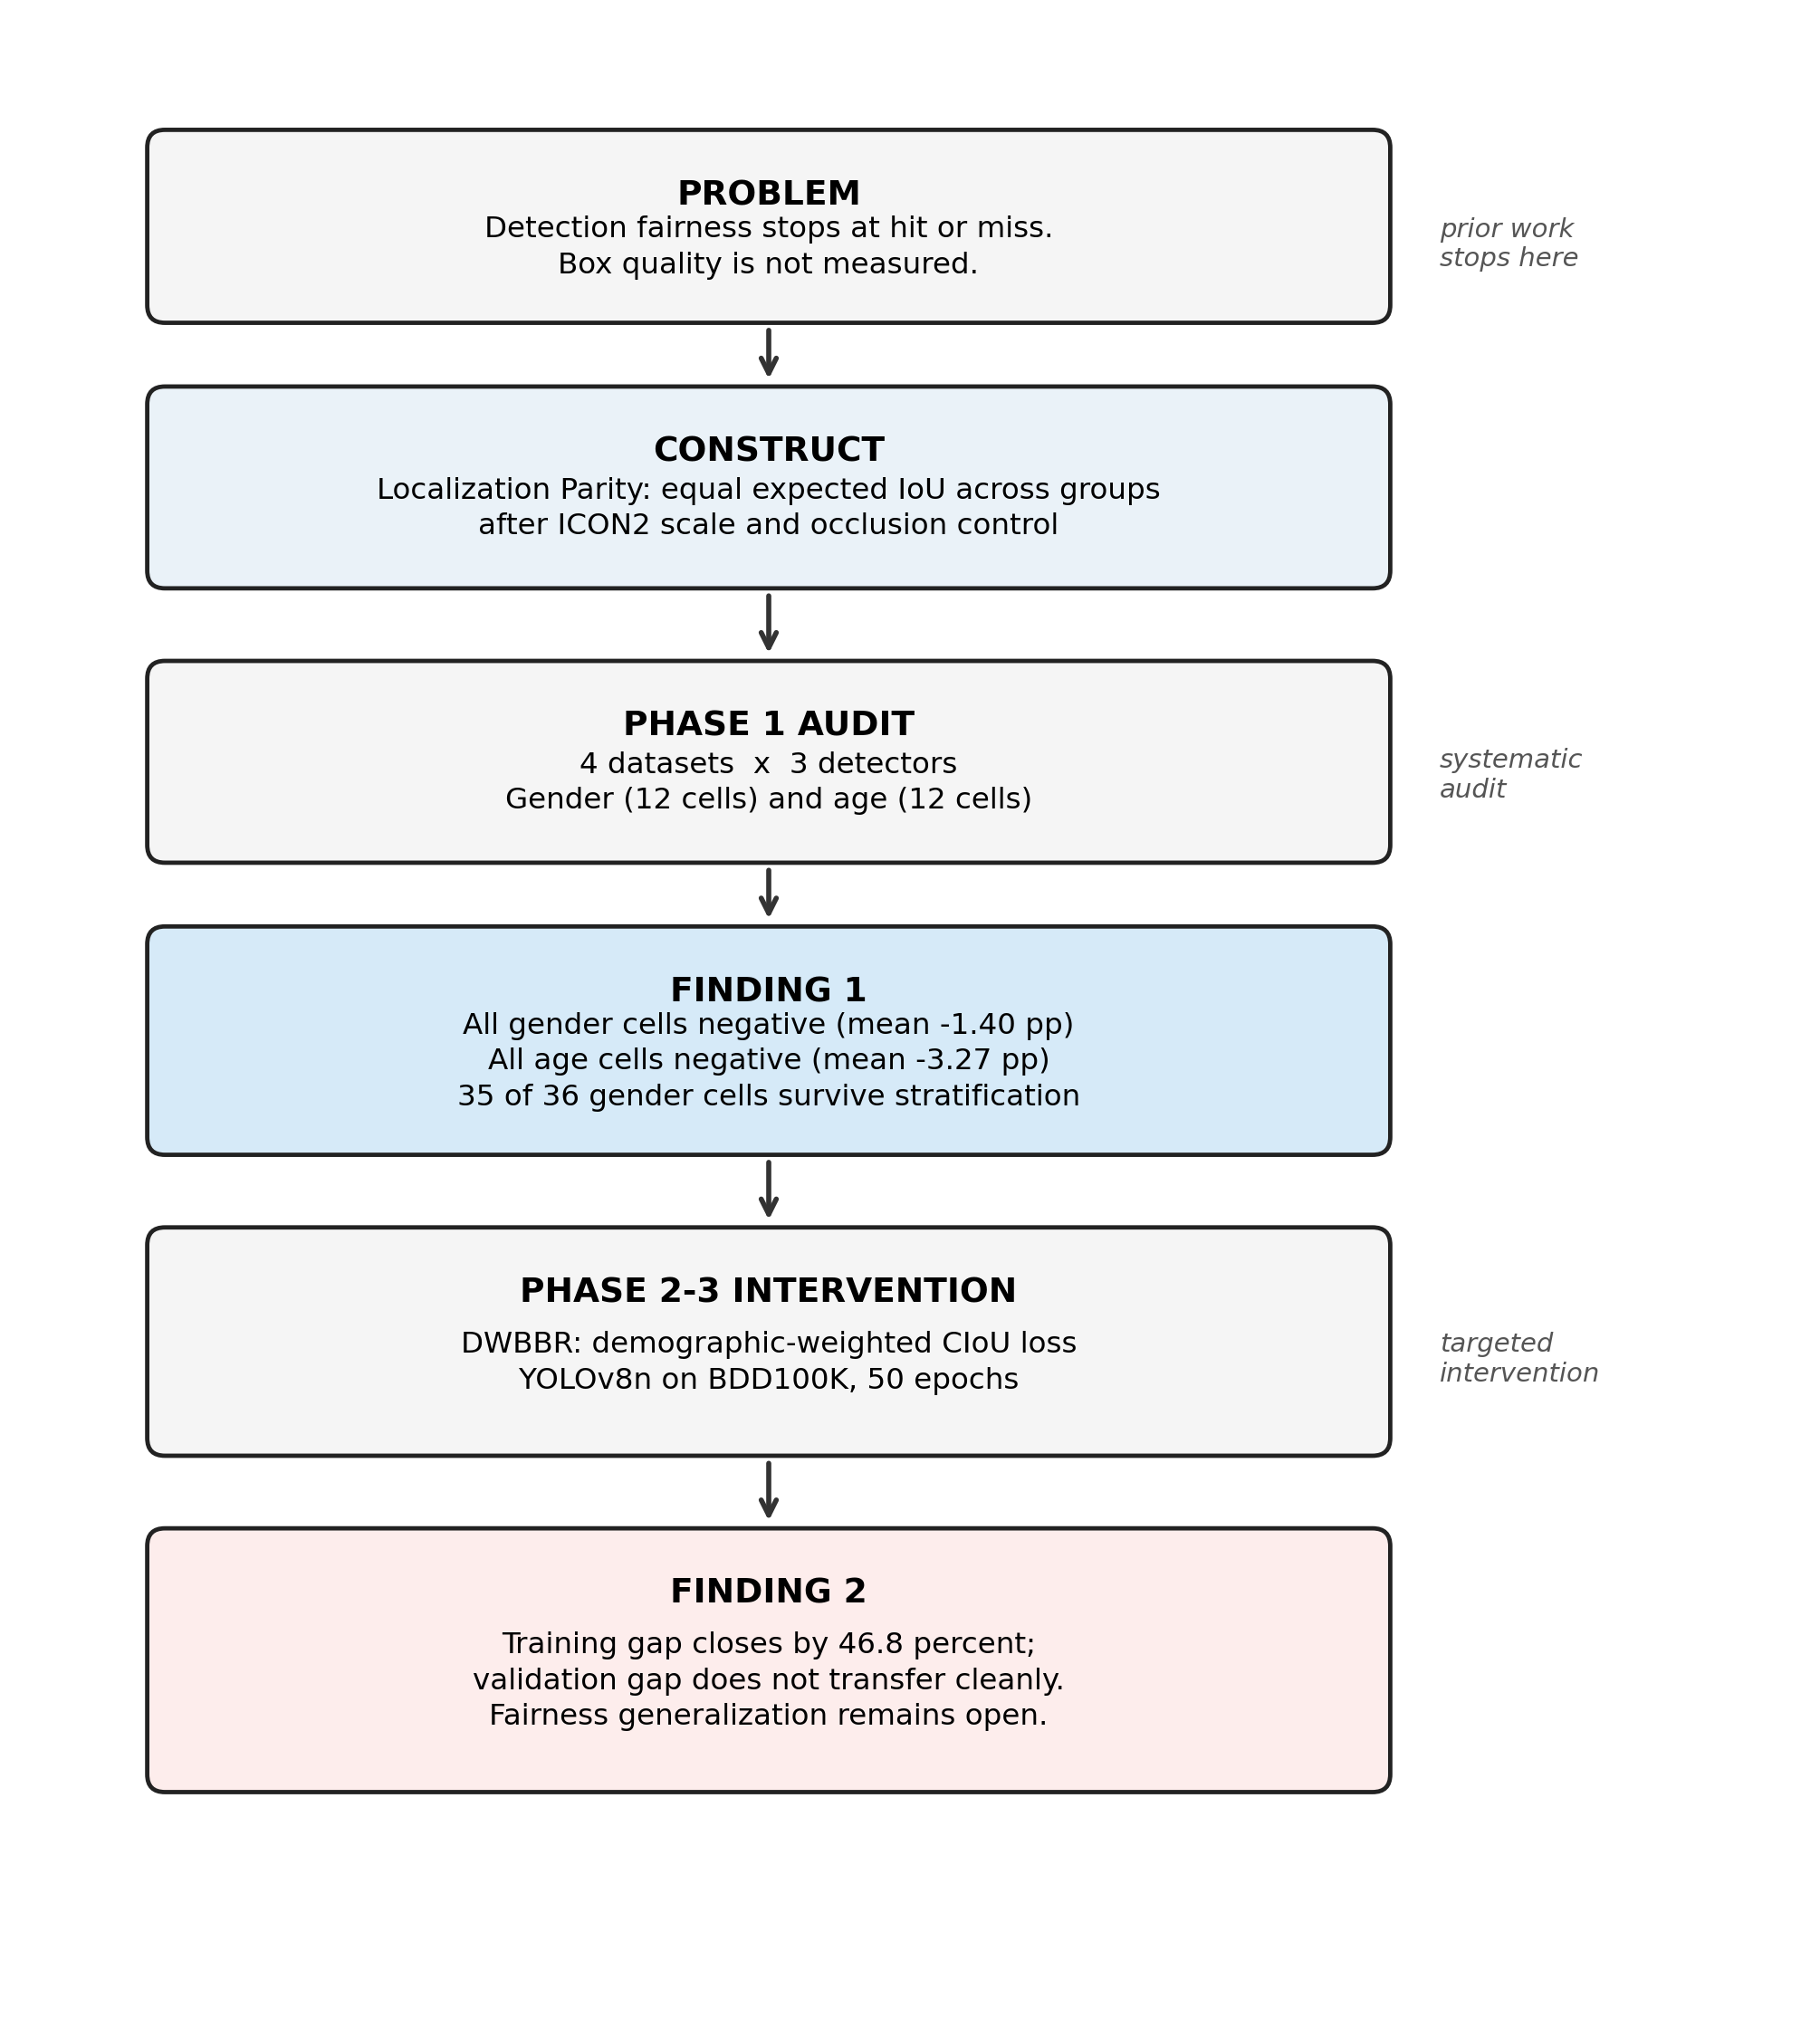
\includegraphics[width=0.88\textwidth]{figures/fig1_framework.png}
\caption{Conceptual framework. Phase~1 audits Localization Parity across four
datasets and three detectors under ICON$^2$ confounder control. Phase~2 and
Phase~3 test whether DWBBR closes the gap and reveal a fairness generalization
barrier.}
\label{fig:framework}
\end{figure}

We evaluate on four pedestrian benchmarks chosen for geographic, sensor, and
lighting diversity: BDD100K~\cite{yu2020bdd100k} (large-scale US dashcam data
with about $100{,}000$ annotated pedestrian boxes and binary male/female
labels), CityPersons~\cite{zhang2017citypersons} (about $19{,}000$ boxes over
$2{,}975$ Cityscapes images with careful occlusion annotation), and
EuroCity-Day together with EuroCity-Night~\cite{braun2019eurocity} (subsets of
EuroCity Persons, covering about $238{,}200$ boxes from $31$ European cities).
Demographic labels for CityPersons and EuroCity use augmented annotations where
available; detections with missing or ambiguous labels are dropped.

The audit covers three detector families with public pretrained weights and no
fine-tuning: YOLOX~\cite{ge2021yolox} (single-stage, anchor-free),
RetinaNet~\cite{lin2017focal} (single-stage, anchor-based), and Cascade
R-CNN~\cite{cai2021cascade} (two-stage, with cascaded IoU refinement). The
mitigation experiments use YOLOv8n as a lightweight trainable backbone. The two
protected attributes are gender (female vs.\ male) and age (child vs.\ adult).
Race and skin tone are excluded because an earlier pilot lacked sufficient
labeled sample size and used categories too coarse for reliable inference.

Predictions are matched to ground truth by greedy, confidence-sorted IoU
assignment; matches with IoU\,$\geq$\,$0.5$ enter the LP analysis. The primary
confounder is object scale (box height), because female and child pedestrians
tend to occupy smaller image regions. Following ICON$^2$, we bin ground-truth
instances within each dataset into short ($\leq$33rd height percentile), medium
(34th--66th), and tall ($\geq$67th) strata, then recompute per-group mean IoU
inside each bin. Within each cell and stratum we compare group IoU distributions
with the two-sided Mann--Whitney $U$ test at $p<0.05$.

Both DWBBR and an identically configured baseline (unweighted YOLOv8n) are
trained on a $1{,}693$-image BDD100K subset with reliable gender labels
($64.8\%$ male and $35.2\%$ female), for $50$ epochs, batch size~$8$, image size
$416\times416$, and $\mathrm{lr}_0=0.01$ with cosine decay on a single NVIDIA
RTX~3050. Validation uses a disjoint $423$-image subset. We replicate with seeds
$\{42,123,7\}$ and select the checkpoint with the best overall validation CIoU
unless otherwise noted.

%% =====================================================================
\section{Experimental Results}
\label{sec:results}
%% =====================================================================

\subsection{Localization Parity Audit}
\label{sec:audit}

Female pedestrians receive lower mean IoU than male pedestrians in all twelve
dataset and detector cells (mean gap $-1.40$\,pp; eleven of twelve significant).
The lone non-significant cell is CityPersons with Cascade~R-CNN ($-0.49$\,pp,
$p=0.11$). BDD100K shows the most consistent gaps ($-2.16$, $-2.02$, and
$-2.32$\,pp), and EuroCity-Night is comparably severe. Children receive lower
mean IoU than adults in all twelve cells as well (mean $-3.27$\,pp; eleven of
twelve significant), roughly double the gender gaps, with EuroCity-Night again
the harshest setting. Tables~\ref{tab:gender} and~\ref{tab:age} and
Figure~\ref{fig:audit} report every cell. Under ICON$^2$ scale stratification
the gender gap survives in $35$ of $36$ cells (mean $-1.43$\,pp) and the age gap
in $24$ of $30$ within-scale cells, so the disparities are not reducible to
women and children occupying smaller image regions.

\begin{table}[!ht]
\caption{Phase~1 LP audit, gender axis. Gap $=$ female minus male mean IoU (pp).
$\dagger$: $p<0.05$, Mann--Whitney~$U$.}
\label{tab:gender}
\centering
\setlength{\tabcolsep}{5pt}
\begin{tabular}{llc}
\toprule
Dataset & Detector & Gap (pp) \\
\midrule
BDD100K & YOLOX & $-2.16^\dagger$ \\
BDD100K & RetinaNet & $-2.02^\dagger$ \\
BDD100K & Cascade R-CNN & $-2.32^\dagger$ \\
CityPersons & YOLOX & $-0.98^\dagger$ \\
CityPersons & RetinaNet & $-0.71^\dagger$ \\
CityPersons & Cascade R-CNN & $-0.49$ \\
EuroCity-Day & YOLOX & $-0.67^\dagger$ \\
EuroCity-Day & RetinaNet & $-0.65^\dagger$ \\
EuroCity-Day & Cascade R-CNN & $-0.98^\dagger$ \\
EuroCity-Night & YOLOX & $-1.81^\dagger$ \\
EuroCity-Night & RetinaNet & $-2.47^\dagger$ \\
EuroCity-Night & Cascade R-CNN & $-1.59^\dagger$ \\
\midrule
\multicolumn{2}{l}{Mean} & $-1.40$ \\
\bottomrule
\end{tabular}
\end{table}

\begin{table}[!ht]
\caption{Phase~1 LP audit, age axis. Gap $=$ child minus adult mean IoU (pp).
$\dagger$: $p<0.05$, Mann--Whitney~$U$.}
\label{tab:age}
\centering
\setlength{\tabcolsep}{5pt}
\begin{tabular}{llc}
\toprule
Dataset & Detector & Gap (pp) \\
\midrule
BDD100K & YOLOX & $-1.92^\dagger$ \\
BDD100K & RetinaNet & $-1.64$ \\
BDD100K & Cascade R-CNN & $-2.83^\dagger$ \\
CityPersons & YOLOX & $-2.91^\dagger$ \\
CityPersons & RetinaNet & $-3.11^\dagger$ \\
CityPersons & Cascade R-CNN & $-3.48^\dagger$ \\
EuroCity-Day & YOLOX & $-4.55^\dagger$ \\
EuroCity-Day & RetinaNet & $-2.49^\dagger$ \\
EuroCity-Day & Cascade R-CNN & $-3.17^\dagger$ \\
EuroCity-Night & YOLOX & $-4.35^\dagger$ \\
EuroCity-Night & RetinaNet & $-4.34^\dagger$ \\
EuroCity-Night & Cascade R-CNN & $-4.44^\dagger$ \\
\midrule
\multicolumn{2}{l}{Mean} & $-3.27$ \\
\bottomrule
\end{tabular}
\end{table}

\begin{figure}[!ht]
\centering
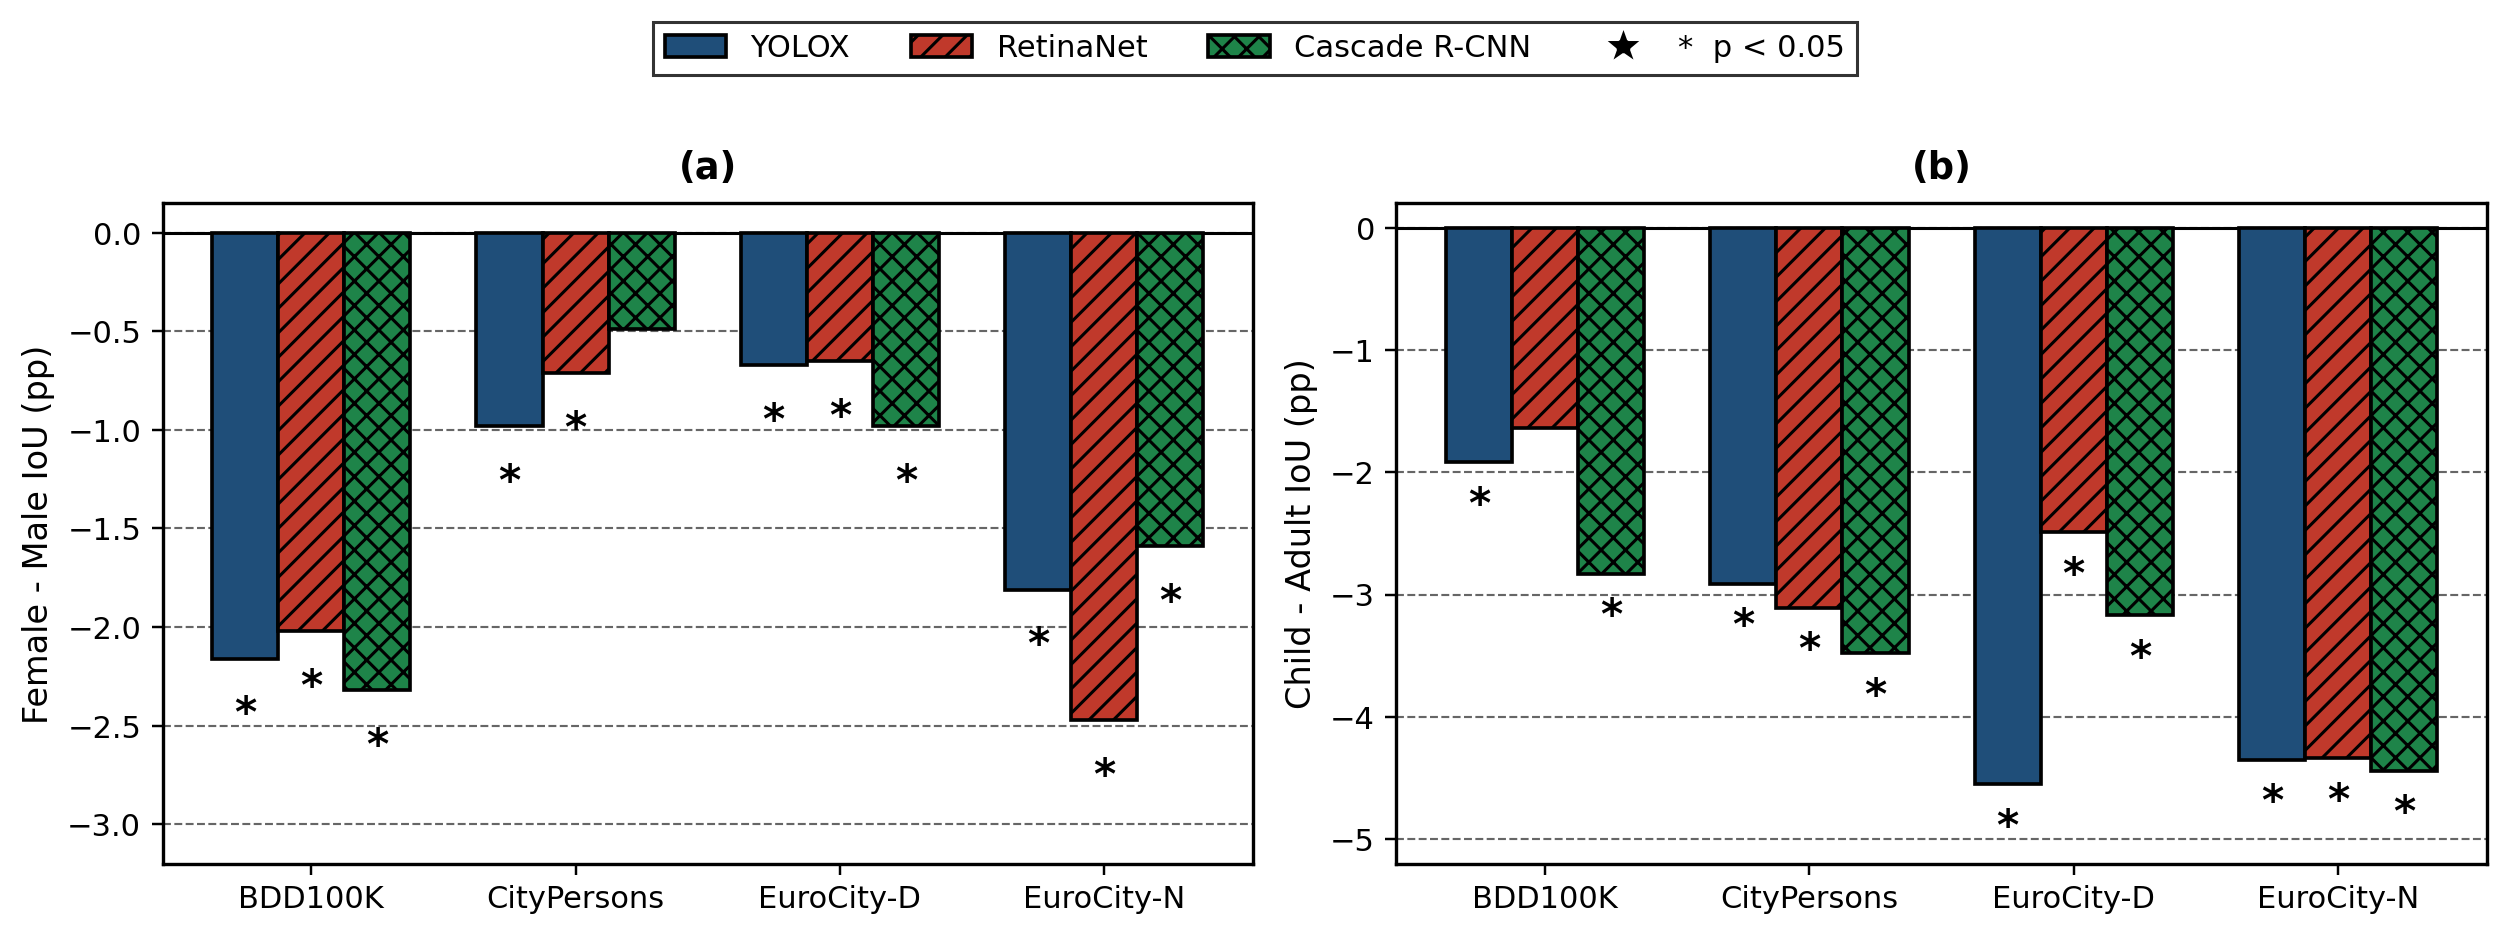
\includegraphics[width=0.95\textwidth]{figures/fig2_audit.png}
\caption{Phase~1 LP audit: gender gaps (a) and age gaps (b) across four datasets
and three detectors. Asterisks mark $p<0.05$.}
\label{fig:audit}
\end{figure}

\FloatBarrier

\subsection{DWBBR Intervention}
\label{sec:intervention}

On the training set, DWBBR behaves as intended
(Figure~\ref{fig:training}): the female-to-male CIoU gap narrows from
$-2.82$\,pp at epoch~$1$ to $-1.50$\,pp at epoch~$50$ ($46.8\%$ relative
reduction), while the female loss weight drifts toward parity as the per-group
IoU ratio improves.

\begin{figure}[!ht]
\centering
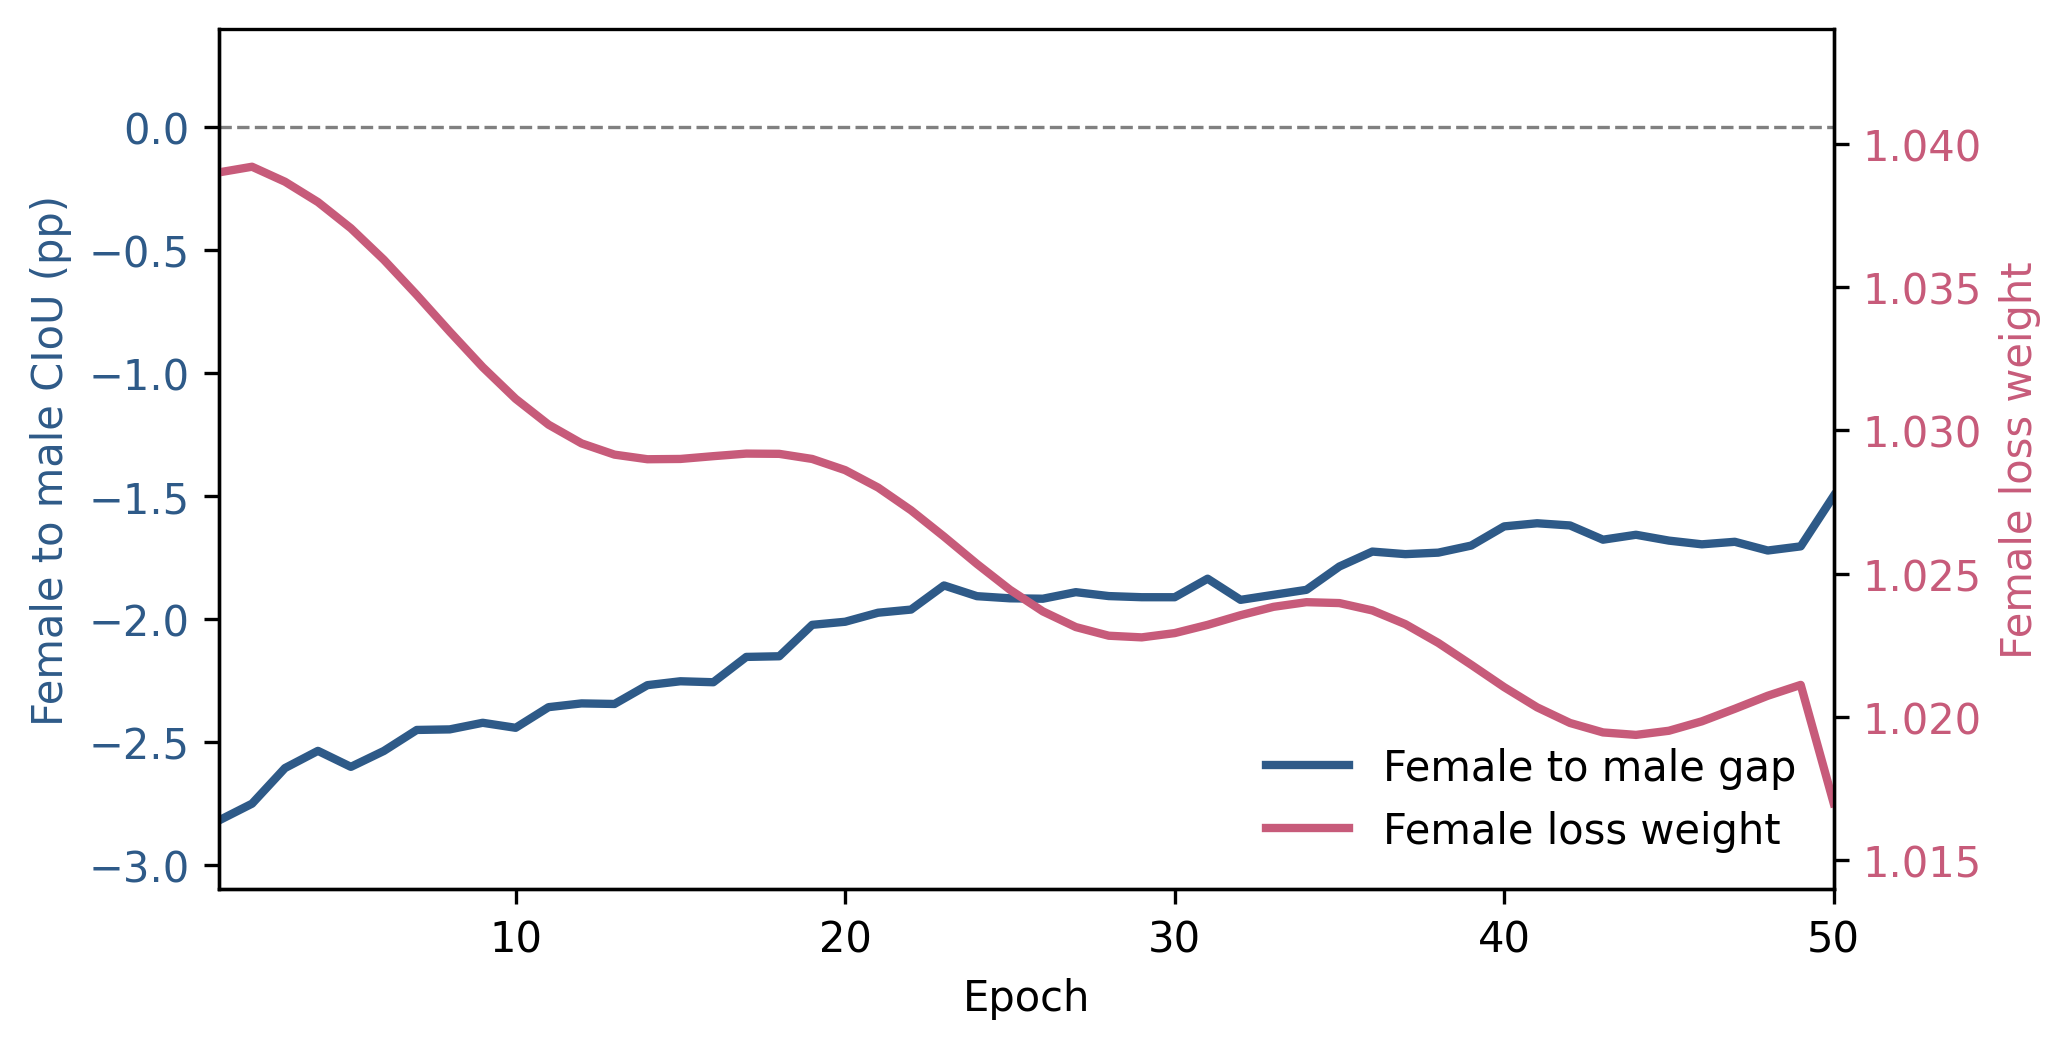
\includegraphics[width=0.70\textwidth]{figures/fig3_training.png}
\caption{DWBBR training dynamics: LP gap convergence over $50$ epochs on
BDD100K.}
\label{fig:training}
\end{figure}

On held-out data the picture changes (Table~\ref{tab:val},
Figure~\ref{fig:val}). Under the primary seed, DWBBR female CIoU is $0.7715$
against baseline $0.7790$; the female-to-male gap widens from $-1.52$\,pp
(baseline) to $-2.74$\,pp (DWBBR). A one-sided Mann--Whitney test finds no
significant female improvement ($p=0.71$). Across three seeds the mean
validation gap moves from $-1.78\pm0.48$\,pp (baseline) to
$-1.36\pm0.63$\,pp (DWBBR), a $23.6\%$ mean reduction accompanied by higher
variance and unstable best-checkpoint epochs ($\{15,17,21\}$ for DWBBR versus
$\{34,17,24\}$ for baseline). DWBBR therefore closes the training LP gap, yet
the improvement does not transfer cleanly: variance rises, checkpoint selection
becomes unstable, and under the primary seed the validation gap worsens. This
aligns with known limits of group reweighting under train--test demographic
shift~\cite{sagawa2020dro}. We report it as a fairness generalization gap rather
than as a claim that all mitigations must fail.
Figure~\ref{fig:qual} shows qualitative Localization Parity violations on
BDD100K.

\begin{table}[!ht]
\caption{Validation CIoU by group on the BDD100K validation subset ($423$
images). Gap $=$ weaker group minus reference group (pp). Multi-seed means use
seeds $\{42,123,7\}$.}
\label{tab:val}
\centering
\setlength{\tabcolsep}{3.5pt}
\begin{tabular}{llcccc}
\toprule
Group & Model & $n$ & CIoU & 95\% CI & Gap (pp) \\
\midrule
Male & Baseline & 555 & 0.7942 & -- & -- \\
Female & Baseline & 376 & 0.7790 & $[0.768,0.790]$ & $-1.52$ \\
Male & DWBBR & 555 & 0.7990 & -- & -- \\
Female & DWBBR & 374 & 0.7715 & $[0.760,0.783]$ & $-2.74$ \\
\midrule
\multicolumn{5}{l}{Mean female to male, baseline} & $-1.78\pm0.48$ \\
\multicolumn{5}{l}{Mean female to male, DWBBR} & $-1.36\pm0.63$ \\
\bottomrule
\end{tabular}
\end{table}

\begin{figure}[!ht]
\centering
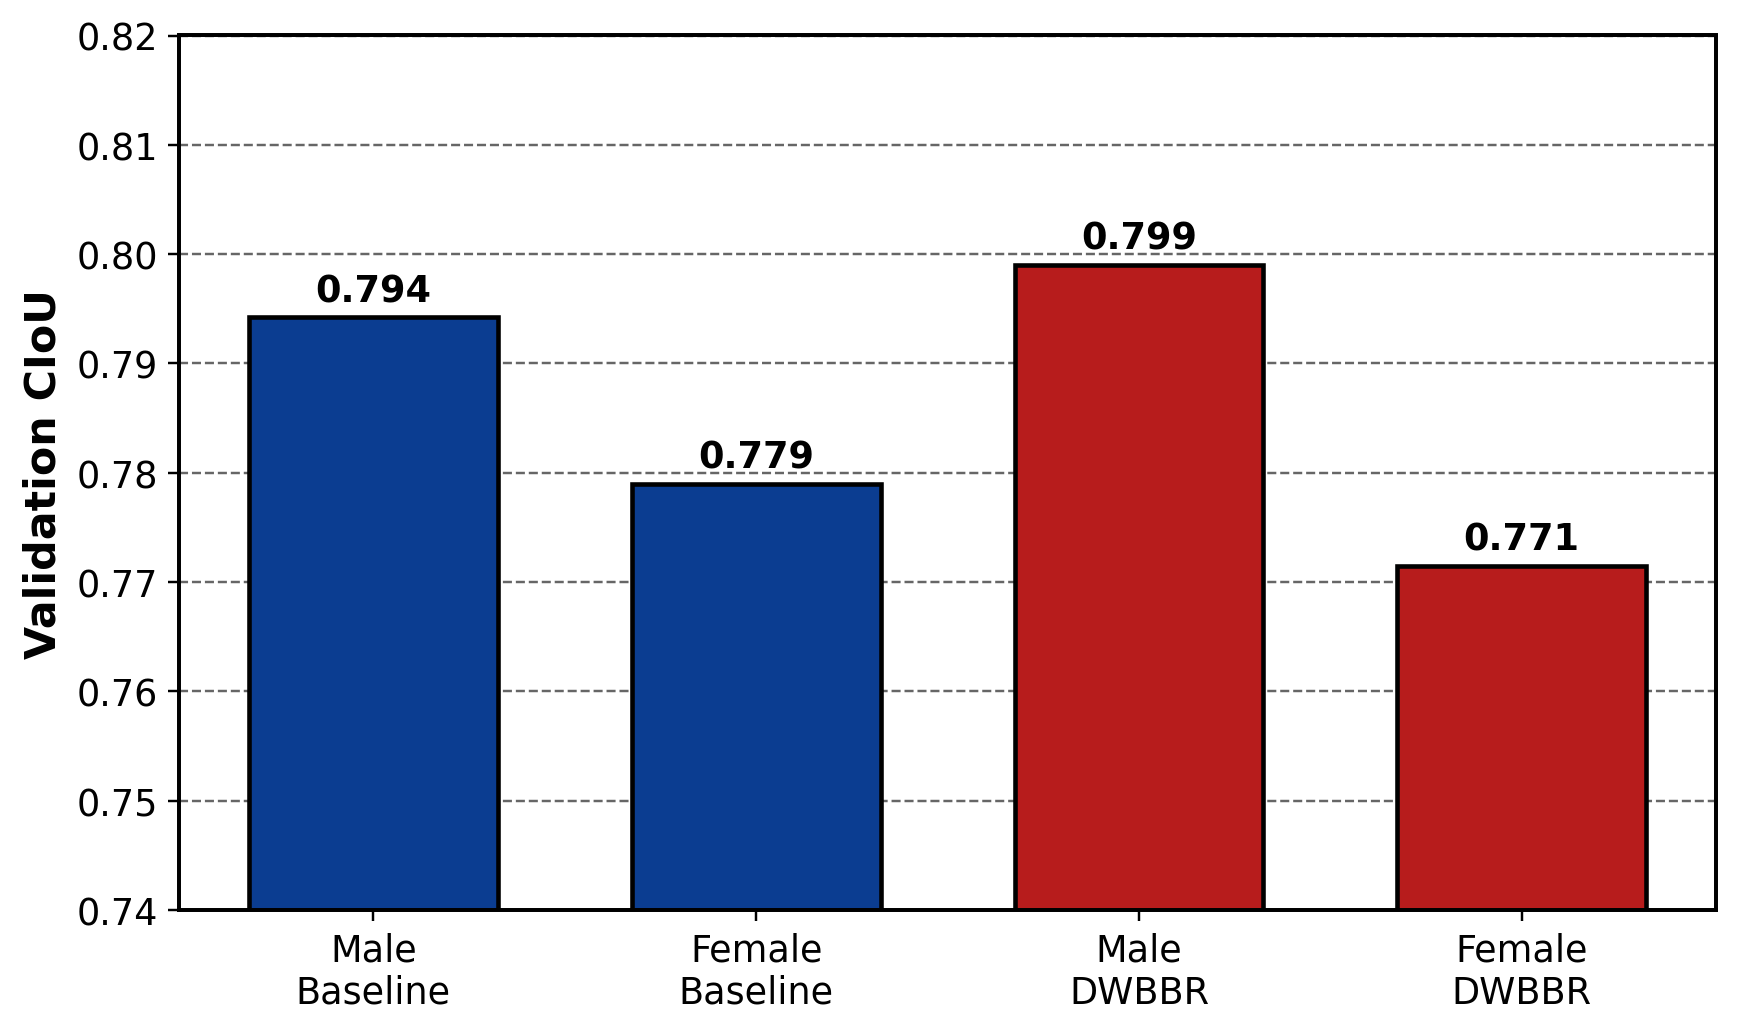
\includegraphics[width=0.58\textwidth]{figures/fig4_validation.png}
\caption{Validation-set CIoU for DWBBR and the baseline, by demographic group.}
\label{fig:val}
\end{figure}

\begin{figure}[!ht]
\centering
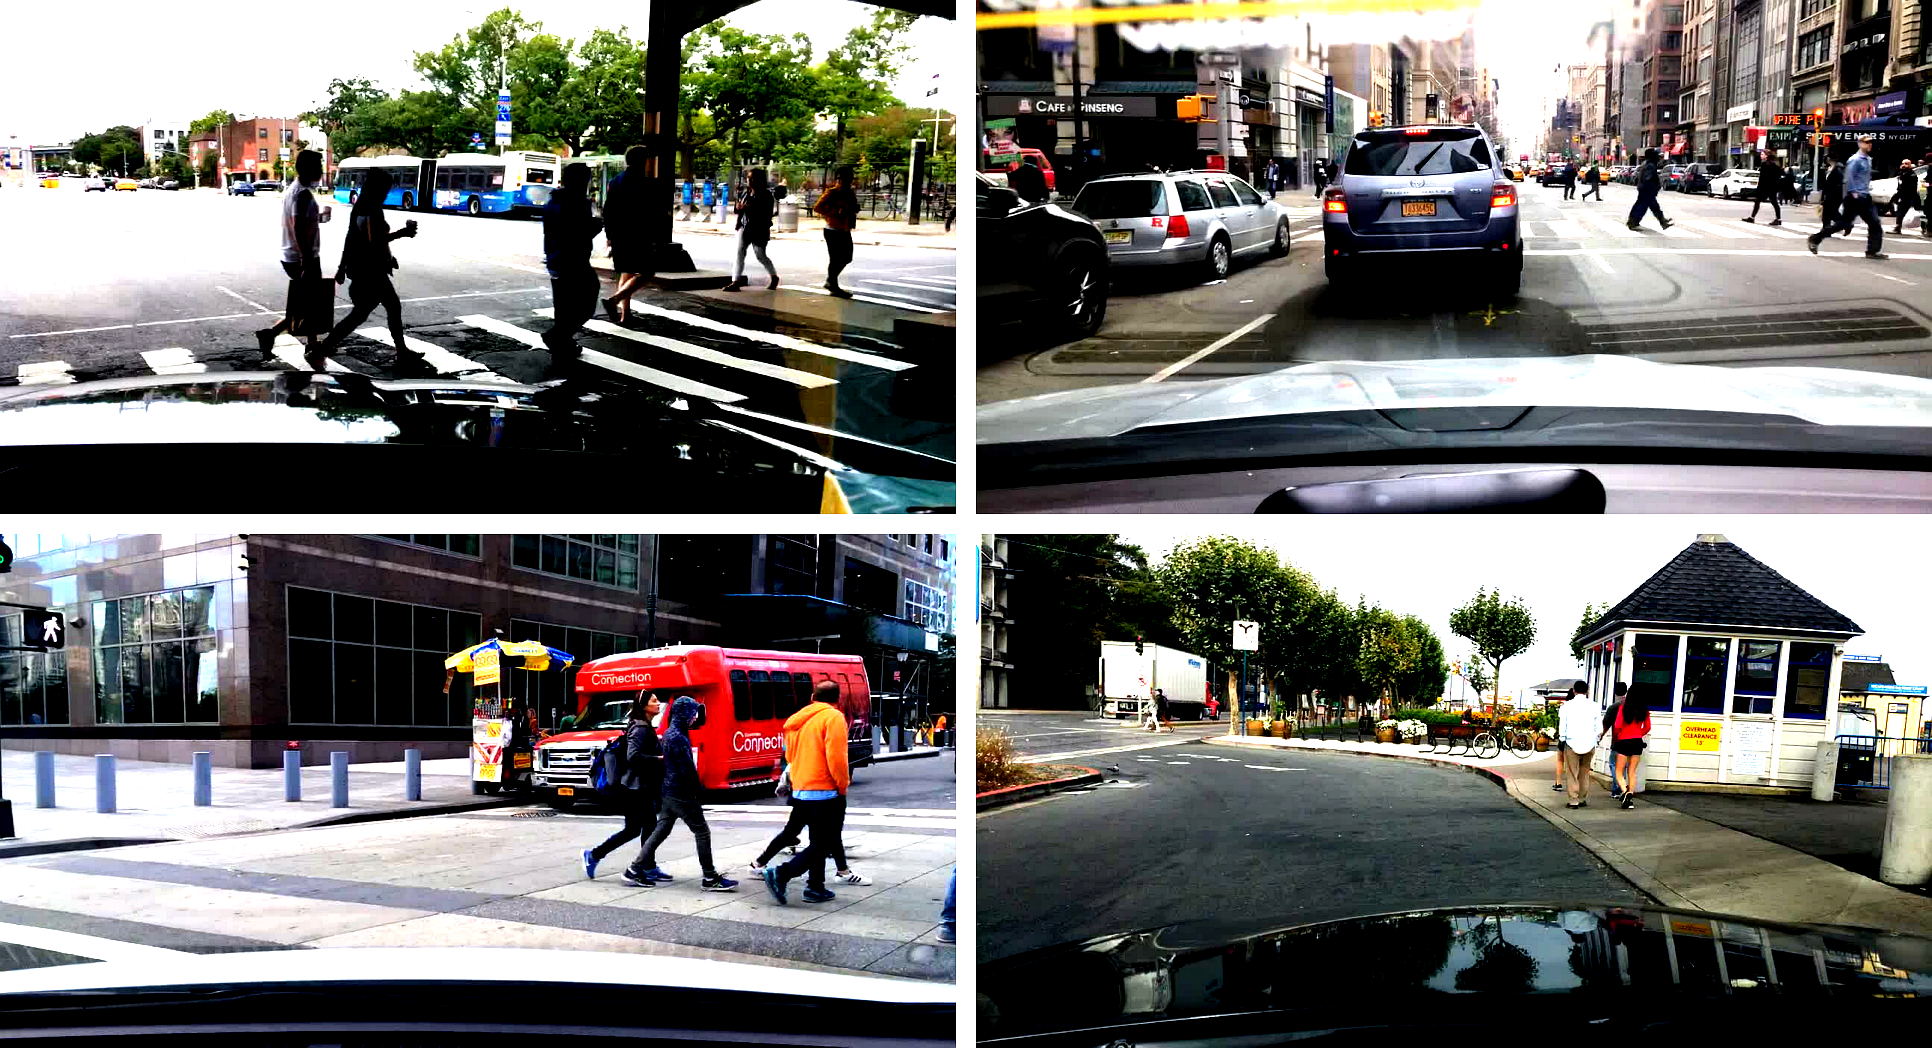
\includegraphics[width=0.82\textwidth]{figures/fig5_qualitative.png}
\caption{Qualitative Localization Parity violations on BDD100K. Female
pedestrians more often receive looser predicted boxes than male pedestrians in
comparable scenes.}
\label{fig:qual}
\end{figure}

\FloatBarrier

Demographic labels in BDD100K are third-party visual inferences with binary
gender, no self-identification, and undocumented annotation guidelines, raising
consent and inclusivity concerns~\cite{schumann2021step}. LP is a proxy for
box-quality fairness rather than a guarantee of equal downstream risk, and
fairer localization can reduce collision risk while also improving
re-identification. We publish because we judge the near-term safety benefit to
outweigh that dual-use risk. The study examines only gender and age; race,
skin tone, disability, body type, and intersectional analyses remain open.

%% =====================================================================
\section{Conclusion}
\label{sec:conclusion}
%% =====================================================================

Localization Parity addresses a previously unmeasured fairness gap in pedestrian
detection: after a person is found, existing audits ignore how tightly the box
fits, even though box geometry drives distance, trajectory, and braking
estimates. This paper contributes a formal LP criterion, the first
confounder-controlled multi-dataset and multi-detector audit of continuous IoU
disparities on gender and age, and a demographic-weighted regression
intervention. Across four datasets and three detector families, female and child
pedestrians receive systematically lower IoU boxes (mean gaps $-1.40$\,pp and
$-3.27$\,pp), and the gaps survive scale stratification, confirming that the
disparity is not explained by object size alone.

Future work should evaluate DWBBR across datasets and architectures, adopt
fairness-aware checkpoint selection, compare stronger DRO and oversampling
baselines, extend audits to skin tone and intersectional groups with higher-
quality labels, and quantify how $1$--$3$\,pp IoU gaps propagate into planning
decisions.

\paragraph{Acknowledgments.}
We thank the PanAfriCon AI 2026 Program Committee and reviewers for constructive
feedback.

\FloatBarrier
\clearpage

\begin{thebibliography}{16}
\small
\setlength{\itemsep}{0.08em}
\setlength{\parsep}{0pt}
\setlength{\parskip}{0pt}

\bibitem{agarwal2019fair}
Agarwal, A., Dud{\'i}k, M., Wu, Z.S.: Fair regression: Quantitative definitions
  and reduction-based algorithms. Proceedings of the International Conference
  on Machine Learning (ICML) (2019)

\bibitem{brandao2019age}
Brandao, M.: Age and gender bias in pedestrian detection algorithms. arXiv
  preprint arXiv:1906.10490 (2019)

\bibitem{braun2019eurocity}
Braun, M., Krebs, S., Flohr, F.B., Gavrila, D.M.: {EuroCity Persons}: A novel
  benchmark for person detection in traffic scenes. IEEE Transactions on
  Pattern Analysis and Machine Intelligence \textbf{41}(8), 1844--1861 (2019)

\bibitem{cai2021cascade}
Cai, Z., Vasconcelos, N.: Cascade {R-CNN}: High quality object detection and
  instance segmentation. IEEE Transactions on Pattern Analysis and Machine
  Intelligence \textbf{43}(5), 1483--1498 (2021)

\bibitem{calders2010discrimination}
Calders, T., Verwer, S.: Three naive {Bayes} approaches for discrimination-free
  classification. In: Data Mining and Knowledge Discovery (2010)

\bibitem{ge2021yolox}
Ge, Z., Liu, S., Wang, F., Li, Z., Sun, J.: {YOLOX}: Exceeding {YOLO} series in
  2021. arXiv preprint arXiv:2107.08430 (2021)

\bibitem{hardt2016equality}
Hardt, M., Price, E., Srebro, N.: Equality of opportunity in supervised
  learning. In: Advances in Neural Information Processing Systems (NeurIPS)
  (2016)

\bibitem{khoshkdahan2025pose}
Khoshkdahan, M., Akbari, A., Akbari, A., Zhang, X.: Beyond overall accuracy:
  Pose- and occlusion-driven fairness analysis in pedestrian detection for
  autonomous driving. arXiv preprint (2025)

\bibitem{li2025bias}
Li, X., Chen, Z., Zhang, J.M., Sarro, F., Zhang, Y., Liu, X.: Bias behind the
  wheel: Fairness testing of autonomous driving systems. ACM Transactions on
  Software Engineering and Methodology \textbf{34}(3), 1--24 (2025)

\bibitem{lin2017focal}
Lin, T.Y., Goyal, P., Girshick, R., He, K., Doll{\'a}r, P.: Focal loss for
  dense object detection. In: Proceedings of the IEEE International Conference
  on Computer Vision (ICCV). pp. 2980--2988 (2017)

\bibitem{sagawa2020dro}
Sagawa, S., Koh, P.W., Hashimoto, T.B., Liang, P.: Distributionally robust
  neural networks for group shifts: On the importance of regularization for
  worst-case generalization. In: International Conference on Learning
  Representations (ICLR) (2020)

\bibitem{schumann2021step}
Schumann, C., Wang, S., Russakovsky, O., Sohl-Dickstein, J., Moritz, P., Forde,
  J.: A step toward more inclusive people annotations for fairness. In:
  Proceedings of the AAAI/ACM Conference on AI, Ethics, and Society (2021)

\bibitem{sudhakar2023icon2}
Sudhakar, S., Prabhu, V., Russakovsky, O., Hoffman, J.: {ICON}$^2$: Reliably
  benchmarking predictive inequity in object detection. In: Proceedings of the
  IEEE/CVF Conference on Computer Vision and Pattern Recognition Workshops
  (CVPRW) (2023)

\bibitem{wilson2019predictive}
Wilson, B., Hoffman, J., Morgenstern, J.: Predictive inequity in object
  detection. arXiv preprint arXiv:1902.11097 (2019)

\bibitem{yu2020bdd100k}
Yu, F., Chen, H., Wang, X., Xian, W., Chen, Y., Liu, F., Madhavan, V., Darrell,
  T.: {BDD100K}: A diverse driving dataset for heterogeneous multitask
  learning. In: Proceedings of the IEEE/CVF Conference on Computer Vision and
  Pattern Recognition (CVPR). pp. 2636--2645 (2020)

\bibitem{zhang2017citypersons}
Zhang, S., Benenson, R., Schiele, B.: {CityPersons}: A diverse dataset for
  pedestrian detection. In: Proceedings of the IEEE Conference on Computer
  Vision and Pattern Recognition (CVPR). pp. 3213--3221 (2017)

\end{thebibliography}

\end{document}
